\documentclass[12pt, a4paper,titlepage]{article}
\usepackage{ae}
\usepackage{lmodern}
\usepackage{amsfonts}
\usepackage{amsmath}
\usepackage{amssymb}
\numberwithin{equation}{section}
\numberwithin{figure}{section}
\usepackage{epsf}
\usepackage{epsfig}
\usepackage{graphicx}
%\usepackage[margin=2cm]{geometry}
\usepackage[T1]{fontenc}
\usepackage[english]{babel}

%\usepackage{showkeys}
\usepackage{setspace}
\frenchspacing
\linespread{1.3}
\usepackage{indentfirst}
\usepackage[utf8]{inputenc}
\usepackage{float}

\usepackage{wrapfig}
\usepackage{subfig}
\usepackage{multirow}
\usepackage{array}
\usepackage{tabularx}
\usepackage[calcwidth]{titlesec}
\usepackage{calc}

\usepackage{geometry}
%kotesre
\geometry{left=2.5cm,right=1.5cm,top=2.0cm,bottom=2.0cm}
%standard
%\geometry{left=2.0cm,right=2.0cm,top=2.0cm,bottom=2.0cm}

\newcommand*{\Resize}[2]{\resizebox{#1}{!}{$#2$}}%


\usepackage[pdftex]{hyperref}
	\hypersetup{colorlinks=true,
		pdfstartview=FitV,
		linkcolor=black,
		unicode=true,
		citecolor=black,
		urlcolor=black
		pdfauthor={Galgóczi Gábor, galgoczi.gabor@wigner.mta.hu},
		pdfsubject={TDK dolgozat},
		pdftitle={}
	}
	
	%\usepackage{biblatex}

%\usepackage[dvips]{graphicx}
%\usepackage{ucs}
%\usepackage[latin2]{inputenc}
%\usepackage{t1enc}
%\def\magyarOptions{defaults=prettiest}
%\usepackage[magyar]{babel}
%\usepackage{fontenc}
%\usepackage{graphicx}
%\usepackage{float}
%\usepackage{textcomp}
%\usepackage{array}
%\usepackage{tabularx}
%\usepackage{booktabs}
%\usepackage{color}
%\usepackage{ae}
%\usepackage{lmodern}
%\usepackage[margin=2 cm]{geometry}
%\usepackage{wrapfig}
%\usepackage{subfig}
%\usepackage{multirow}

\newcommand{\red}[1]{\textbf{\textcolor{red}{#1}}}
\newcommand{\pink}[1]{\textbf{\textcolor{magenta}{#1}}}
\newcommand{\blue}[1]{\textbf{\textcolor{blue}{#1}}}
\newcommand{\green}[1]{\textbf{\textcolor{green}{#1}}}
\usepackage[none]{hyphenat}
\sloppy
\titleformat{\section}{\large \bf }{\thesection.}{.5 em}{}[\vspace{-0.8 em}\rule{\titlewidth}{1pt}]


\begin{document}

\begin{titlepage}

\begin{center}
\ \\

\vspace{1 cm}
\begin{large}\textbf{Detailed feasibility study of a gamma ray detector system for nanosatellites using GEANT4 simulations}\end{large}\\
\vspace{1 cm}
%\begin{larger}\textbf{BSc szakdolgozat}\\ \end{larger}
%\vspace{0.5 cm}
\textit{\textbf{Galgóczi Gábor$^{*}$, Fizikus MSc szak, 2. évfolyam}}\\
Eötvös Loránd Tudományegyetem, Természettudományi Kar\\
WIGNER Fizikai Kutatóközpont - MTA\\
\vspace{1.5cm}


\begin{figure}[H]
\centering



\includegraphics[width=80.0mm]{images/elte.png}  
\end{figure}


%\begin{figure}
%\centering
%\begin{subfigure}{5\textwidth}
 % \centering
  %\includegraphics[width=4\linewidth]{bme_logo_kicsi.jpg}
%\end{subfigure}%
%\begin{subfigure}{5\textwidth}
 % \centering
  %\includegraphics[width=4\linewidth]{image.jpg}
%\end{subfigure}
%\end{figure}



\vspace{4 cm}
\end{center}

\begin{center}
\begin{tabular}{ll}
\centerline{ Témavezetők: } \\
\centerline{ Norbert Werner (ELTE)}
\end{tabular}
\end{center}
\begin{center}

\vspace{2.5 cm}
\large \textbf {2018}\\
\end{center}
\end{titlepage}
%\doublespacing
\tableofcontents
%\singlespacing
\pagenumbering{roman}



\pagebreak
\pagenumbering{arabic}
\setcounter{page}{1}



%%%%%%%%%%%%%%%%%%%%%%%%%%%%%%%%%%%%%%%%

\section{Introduction}

High energy astrophysics

\subsection{Aim of the simulation}

The main aim of the paper, therefore this thesis is to optimize the scintillators of the CubeSats (miniaturized satellites) in the Constellation Gamma satellites. The second aim is to understand how the material of the CubeSat would affect the gamma photons that the satellite is meant to detect.

\subsection{The Constellation Gamma (ConGa) fleet}

\subsection{The simulated setup}


HAMAMATSU S13360-6050CS

datasheet of QE:
%http://www.hamamatsu.com/resources/pdf/ssd/s13360_series_kapd1052e.pdf

esr foil:
Please check "ESR from 3M" company. e.g.,
%http://multimedia.3m.com/mws/media/466120O/esr.pdf

\subsection{Simulation}

In order to understand how the $\gamma$ photons -- that the CubeSat is meant to detect -- interact with the matter of the satellite simulations are needed. In a simulation it is also possible to determine the optimal geometry that would lead to the best GRB detection. 

The Geometry... XXX TRacking (Geant4) 


The cross section for photoeffect is far the largest by far for low energy gamma photons.
The ionized nuclei and the secondary electrons generates scintillation.

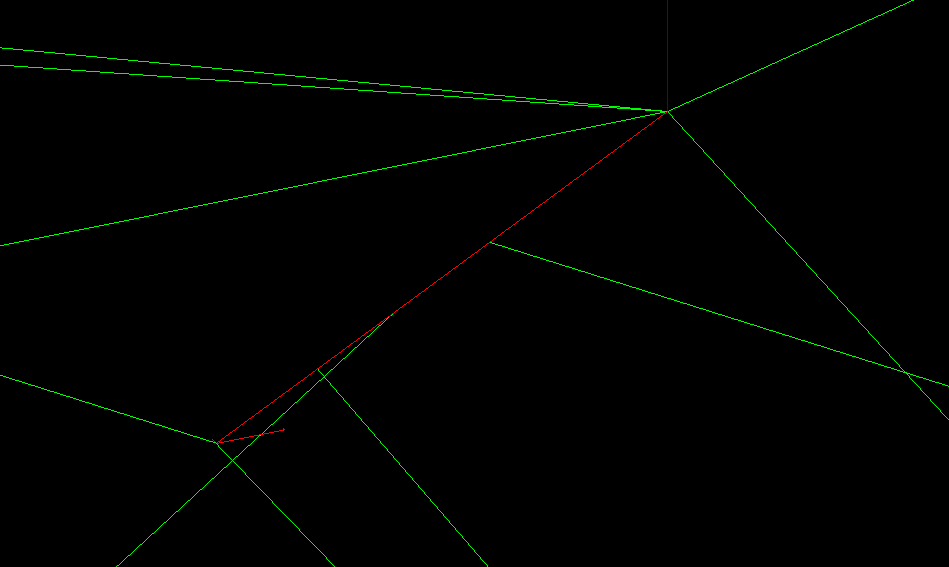
\includegraphics[width=130.0mm]{images/secondary.png}


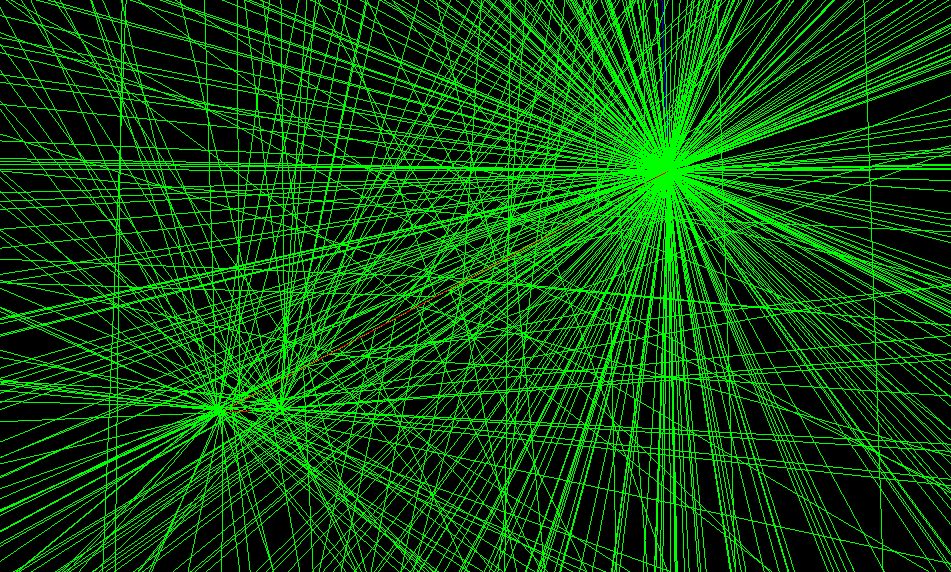
\includegraphics[width=130.0mm]{images/secondary2.png}

Also the nuclei that is ionized by the gamma produces photons.
 
\subsection{Fine tuning the optical parameters}

Most relevant parameters:
\begin{itemize}
\item absoprtion length of the scintillator material
\item scintillation yield
\end{itemize}

\section{Setup}

Size of the scintillator is, the aluminium housing thickness is, the size of the SiPM is...

Parameters of the CsI(Tl) scintillator REF

\begin{itemize}
\item Scintillation yield (Number of photons produced by given keV depleted in the scintillator)
\item The energy spectra of the produced scintillation
\item The time constant of the scintillation photon creation
\item The absorbtion length of the optical photons
\item Birks constant?
\end{itemize}

Optical parameters of the materials and surfaces:
\begin{itemize}
\item Refractive indices of all relevant materials
\item Reflection
\item The detection efficiency of the SiPM detectors
\end{itemize}

\subsection{1 channel setup}

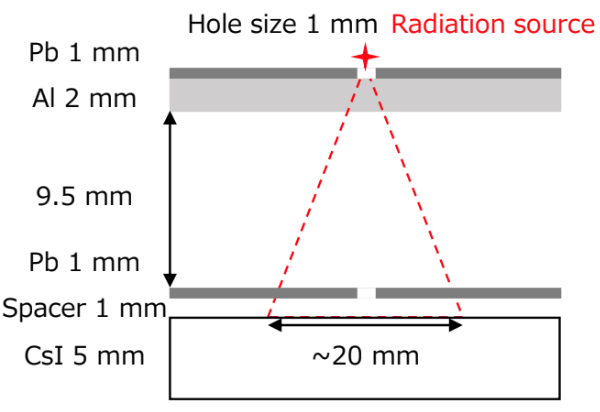
\includegraphics[width=150.0mm]{images/irradiation.png}

\subsection{2 channel read out setup}

\begin{figure}[H]
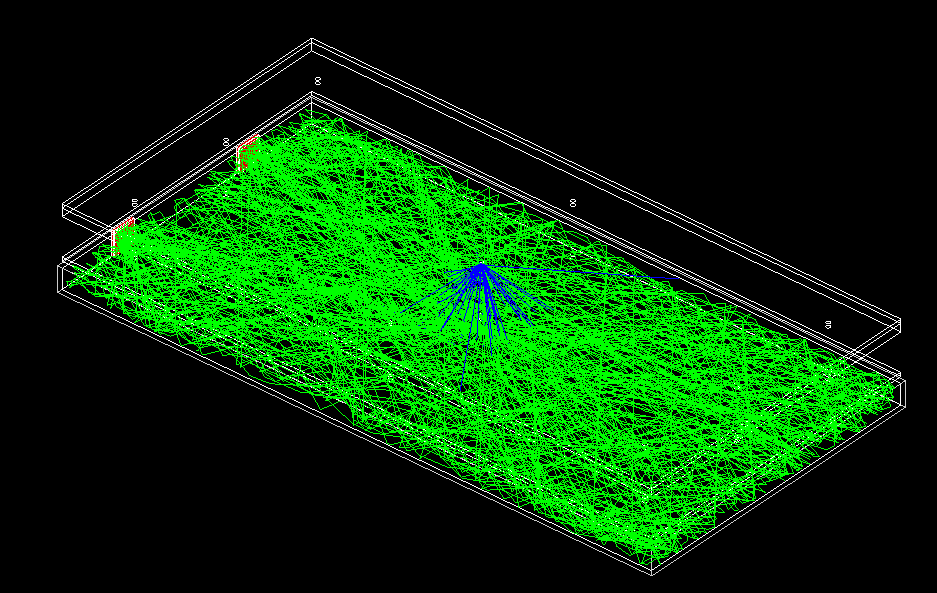
\includegraphics[width=160.0mm]{images/2channel.png}
\caption{Simulation of 100 $\gamma$s emitted from the source. The blue lines represent the track of the $\gamma$s and the green lines represent the track of the optical photons created by scintillation. Only the photons that were detected are drawn.}
\end{figure}



\subsection{The satellite}

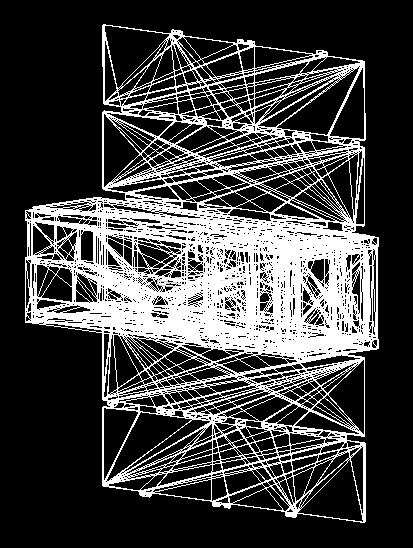
\includegraphics[width=100.0mm]{images/satellite.png}

\begin{table}
\begin{center}
\begin{tabular}{ |c|c|c|c|} 
 \hline
 Name of module & mass [g] & Type of material & Mass ratio [\%]\\\hline
 ADCS &	710	& Aluminum 6061-T6 &	50\\
			& & Copper Electric	& 25 \\
			& &  Glass Borosilicate 	& 25\\\hline
ANT		&  110		& Stainless Steel 	& 50\\
		&  & FR4 Glass-Epoxy sheet	& 50\\\hline
AUX		& 100	& 	FR4 Glass-Epoxy sheet	& 100\\\hline
COM	& 	90	& 	Stainless Steel 	& 2\\
			& 	& Brass Generic		& 25\\
			& 	& Aluminum 7075-T73		& 40\\
			& 	& FR4 Glass-Epoxy sheet	& 	33\\\hline
EPS	& 	750	& 	FR4 Glass-Epoxy sheet		& 25\\
			& 	& Aluminum 6061-T6		& 75\\\hline
OBC	&	50		& FR4 Glass-Epoxy sheet	& 	100\\\hline
STRU	& 	980		& Aluminum 6061-T6	& 	100\\\hline
SP	& 	570		& Solar Panel	& 	100\\\hline
Payload	& 	1100	& 	As you wish	& 	100\\
 \hline
\end{tabular}
\end{center}
\caption{The mass ratio of materials that are used for the satellite}
\end{table}

\begin{table}

\begin{center}
\begin{tabular}{ |c|c|c|c|c|c|c|c|c|c|c|c|c|} 
 \hline
%Material name & El. 1	& El. 1 m.r. & El. 2 & El. 2 m.r. &El.3	& El. 3 m.r. &El. 4	& El. 4 m.r. &El.	5& El. 5 m.r. &El.	6& El. 6 m.r. \\\hline
Material name & &&&&&&&&&&& \\\hline

Aluminum 6061-T6 &	Al & 96.90 &	Mg &	1.20 &	Si &	0.80 &	Fe &	0.70 &	Cu &	0.40 & &\\\hline		
Aluminum 7075-T73 &	Al &	88.60 &	Zn &	6.10 &	Mg &	2.90 &	Cu &	2.00 &	Si &	0.40 & &\\\hline		
%Stainless Steel A2-70  AISI 304 (EN 1.4301) &	Fe &	66.50 &	Cr &	20.00 &	Ni &	10.50	Mn &	2.00 &	Si &	1.00 & &\\\hline		
Stainless Steel &	Fe &	66.50 &	Cr &	20.00 &	Ni &	10.50	&Mn &	2.00 &	Si &	1.00 & &\\\hline		
Copper Electric  &Cu &	100.00 & & & & & & & & & &	\\\hline					
Glass Borosilicate &	Si &	42.10 &	O &	54.80 &	B &	3.10 & & & & & &\\\hline			
FR4 Glass-Epoxy &	Si &	23.39 &	O &	36.02 &	C &	37.04 &	H &	3.55 & & & &\\\hline		
Brass Generic &	Cu &	85.00 &	Zn &	15.00 & & & & & & & &\\\hline						
Solar Panel &	Ge &	38.00 &	Si &	24.00 &	O &	20.00 &	C &	13.00 &	H &	4.00 &	B &	1.00\\\hline
\end{tabular}
\end{center}
\caption{The chemical composition of materials that are used for the satellite}
\end{table}

\pagebreak

\section{Results of the simulation}
\subsection{Comparison of the results of the simulation with experiments}

%ADC / energy calibration from measurement 20170829 illetve az egy chanellel: grb\_status3 

1 channel read out:

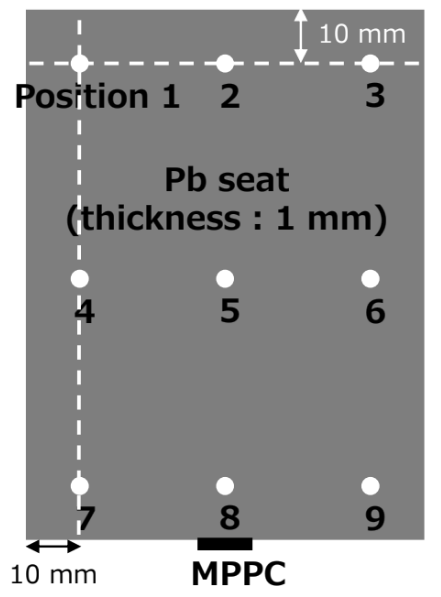
\includegraphics[width=80.0mm]{images/positions.png}

The experimental results:

\begin{center}
\begin{tabular}{ |c|c|c|c|c|c|c|c|c|c| } 
 \hline
  Pos. of source & 1 & 2 & 3 & 4 & 5 & 6 & 7 & 8 & 9 \\ 
  Pos. of main peak & 0.642 & 0.664 & & 70.7 & 0.743 & & 0.598 & &  \\ 
 \hline
\end{tabular}
\end{center}

The parameters set in the simulation: reflectivity: 0.995 and absoprtion length of
40 cm:

\begin{center}
\begin{tabular}{ |c|c|c|c|c|c|c|c|c|c| } 
 \hline
  Pos. of source & 1 & 2 & 3 & 4 & 5 & 6 & 7 & 8 & 9 \\ 
  Pos. of main peak & 0.3389 & 0.3256 & 0.3355 & 0.3521 & 0.3555 & 0.3522 & 0.2060 & 1 & 0.203  \\ 
 \hline
\end{tabular}
\end{center}


The parameters set in the simulation: reflectivity: 0.995 and absoprtion length of 50 cm

\begin{center}
\begin{tabular}{ |c|c|c|c|c|c|c|c|c|c| } 
 \hline
 Pos. of source & 1 & 2 & 3 & 4 & 5 & 6 & 7 & 8 & 9 \\ 
 Pos. of main peak & 0.4013 & 0.3917 & 0.3981 & 0.4045 & 0.4172 & 0.4140 & 0.2580 & 1 & 0.2739\\ 
 \hline
\end{tabular}
\end{center}

Reflectivity of 0.997 and abs. length of 60 cm

\begin{center}
\begin{tabular}{ |c|c|c|c|c|c|c|c|c|c| } 
 \hline
  Pos. of source & 1 & 2 & 3 & 4 & 5 & 6 & 7 & 8 & 9 \\ 
  Pos. of main peak & 0.4588 & 0.4587 & 0.4697 & 0.4734 & 0.4700 & 0.4737 & 0.3388 & 1 & 0.3365  \\ 
 \hline
\end{tabular}
\end{center}




\subsection{X-ray fluorescence}
Histogram without fluorescence, turned out in LXeEMPhysics line 140-159

Histogram with flo

\subsection{Simulation of the cosmic background in space}


\subsection{Optimalization of the scintillator detectors}

\pagebreak
\section{Conclusion}

In order to simulate how the XXX CubeSat would interact with the cosmic background and how sensitive it would be to the GRBs that it is designed to investigate a Geant4 simulation was built.

As the first step, the experimental setup that was used to test the CsI(Tl) scintillator -- the particle detector of the satellite -- was implemented in Geant4. The optical parameters of the simulation were fine tuned by comparing the light yield of the MPPCs that was used to read out the scintillator.

Secondly, the CAD model of the satellite was exported to Geant4. The body of the satellite was divided into 8 modules. The chemical components of these modules were included in the simulation. The scintillator was placed on the side of the satellite.

Thirdly, the effect of cosmic radiation was invastigated by obtaining the energy spectra of cosmic protons and electrons at the XXX altitude of XXX. The satellite was radiated by these particles in Geant4 from all directions to investigate how large the signal of these particles would be. This needs to be minimalized as it versenyez with the signal of gamma particles from GRBs.

Finally, the $\gamma$ absorption of the satellite was invastigated.

\pagebreak

\section{Acknowledgment}

 
\pagebreak

\addcontentsline{toc}{section}{References}
\begin{thebibliography}{99}
\interlinepenalty=10000

\bibitem{tgemadv} C. Shalem, R. Chechik, et al.,\\
Advances in Thick GEM-like gaseous electron multipliers—Part I: atmospheric pressure operation,\\
Nuclear Instruments and Methods in Physics Research A, vol. 558, page 475-489, 2006

\end{thebibliography}

\pagebreak




\end{document}

\begin{figure}[h!]
\centerline{
\includegraphics[width=260pt,angle=0]{images/let_setup.png}}
\caption{Az általam használt OTPC a gázrendszerével, illetve a kiolvasórendszerével együtt}
\end{figure}

Sötét anyag kutatásra jó beveztő:
https://arxiv.org/pdf/1510.02170.pdf
Nuclear physics:
https://indico.fnal.gov/conferenceDisplay.py/abstractBook?confId=8976

%%%%%%%%%%%%%%%
Alkalmazások


M. Pomorski, M. Pfutzner
M. Pomorski et al. Phys. Rev. C 90, 014311 (2014)

Micromegas-os kiolvasás J. B. R. Battat, Nucl. Instr. Meth. A 755(2014)6.

[grid???] U. Titt, V. Dagendorf et al., (Nucl. Instr. Meth. A 477 (2002) 536:	 
grids, pure TEA at low pressure, (electron counting / nano-dosimetry)

%%%%%%%%%%%%%%

Performance of an optical readout GEM-based TPC, L.M.S. Margato a...

optikai úton kiolvasott tpc-k: florian e-mailjéből

LET TPC

radon és polónium energiáira cikkek